\documentclass[assignment1.tex]{subfiles}
\begin{document}

\section*{1η Άσκηση}

Το επίπεδο σώμα εκτείνεται μόνο σε 2 διαστάσεις, στο χωρίο $$D=\left\{(x,y): x\in[0,2], y\in[0,2], x^2+y^2>1, x+y<2\right\}$$ Η μάζα και το κέντρο μάζας του σώματος δίνονται από τα ολοκληρώματα \ref{eq:mass}, \ref{eq:xcm}, \ref{eq:ycm}. Είναι προφανές από τα όρια του χωρίου $D$, ότι οι συντεταγμένες του κέντρου μάζας θα είναι ίσες.

\begin{equation}
m=\int_D 1+x^2+y^2 \mathrm{d}x \mathrm{d}y
\label{eq:mass}
\end{equation}

\begin{equation}
x=\frac{1}{m}\int_D x\left(1+x^2+y^2\right) \mathrm{d}x \mathrm{d}y
\label{eq:xcm}
\end{equation}

\begin{equation}
y=\frac{1}{m}\int_D y\left(1+x^2+y^2\right) \mathrm{d}x \mathrm{d}y
\label{eq:ycm}
\end{equation}

Από αναλυτικό υπολογισμό των ολοκληρωμάτων, που έγινε με χρήση του πακέτου \textlatin{Mathematica}, αναμένεται $m=3.4885$, $x_{cm}=0.84084$ και $y_{cm}=0.84084$. Η μέθοδος της απόρριψης για 10000 δείγματα δίνει τα εξής: $m=3.53\pm0.05$, $x_{cm}=0.833\pm0.013$ και $y_{cm}=0.846\pm0.013$. 

Όπως φαίνεται από τη σύγκριση των τιμών, οι υπολογισμοί \textlatin{Monte Carlo} με τα απόλυτα σφάλματά τους είναι κοντά στις αναλυτικές λύσεις των ολοκληρωματων. Η μικρή διαφορά στην τιμή των συντεταγμένων του κέντρου μάζας οφείλεται στη δειγματοληψία διαφορετικών γεννητριών τυχαίων αριθμών για τα $x$ και $y$. Ωστόσο, το σφάλμα των μέσων τιμών δεν αλλάζει καθώς οι γεννήτριες έχουν τα ίδια χαρακτηριστικά.

Κατά την εκτέλεση του προγράμματος, παράχθηκαν τα σημεία που φαίνονται στο Σχήμα \ref{fig:rejection}.

\begin{figure}[hp]
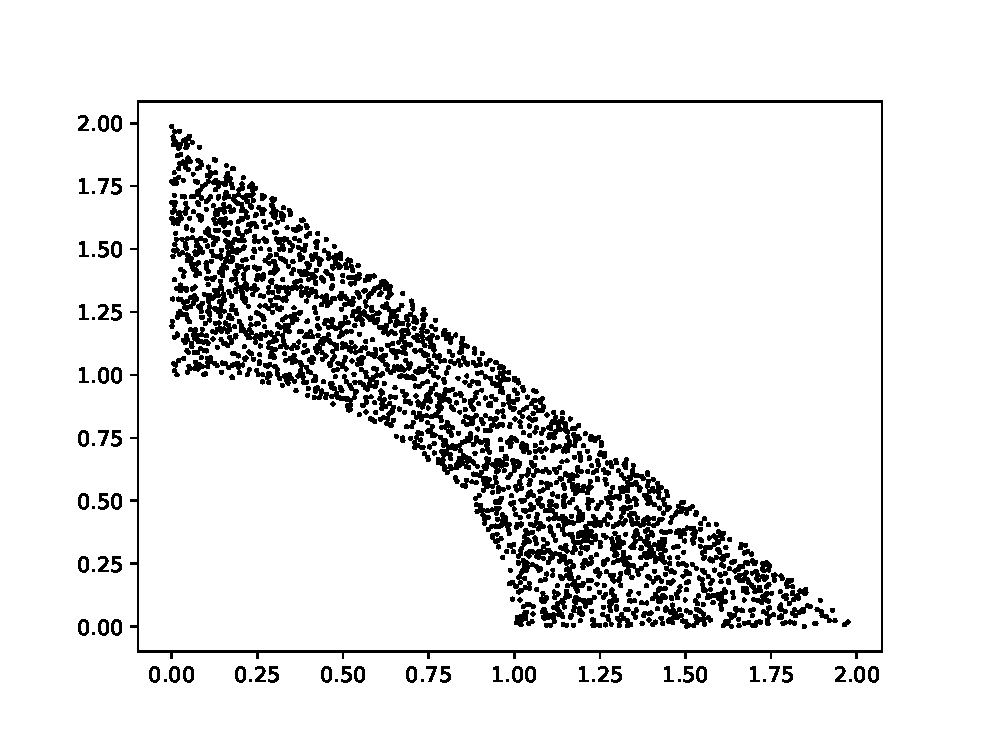
\includegraphics[width=0.9\textwidth]{rejection.eps}
\centering
\caption{Σημεία εκτέλεσης \textlatin{Monte Carlo}}
\label{fig:rejection}
\end{figure} 

\FloatBarrier

Παρακάτω ακολουθεί ο κώδικας που γράφτηκε σε \textlatin{Python} και έγινε χρήση της βιβλιοθήκης \textlatin{Numpy}.

\selectlanguage{english}
\lstinputlisting[style=python, firstline=8]{mc_rejection.py}

\end{document}